\documentclass[thesis-solanki.tex]{files}


\begin{document}

\chapter{Prototype 3}{\label{proto3}}


\section{About this chapter}
This chapter discusses the procedure to infuse multiple search strategies into a \progLang{Prolog} query resolver with monadic unification. 

\david{This chapter is beautifully illustrated by Figure~\vref{fig:architecture-proto-3}.}

\begin{figure}
  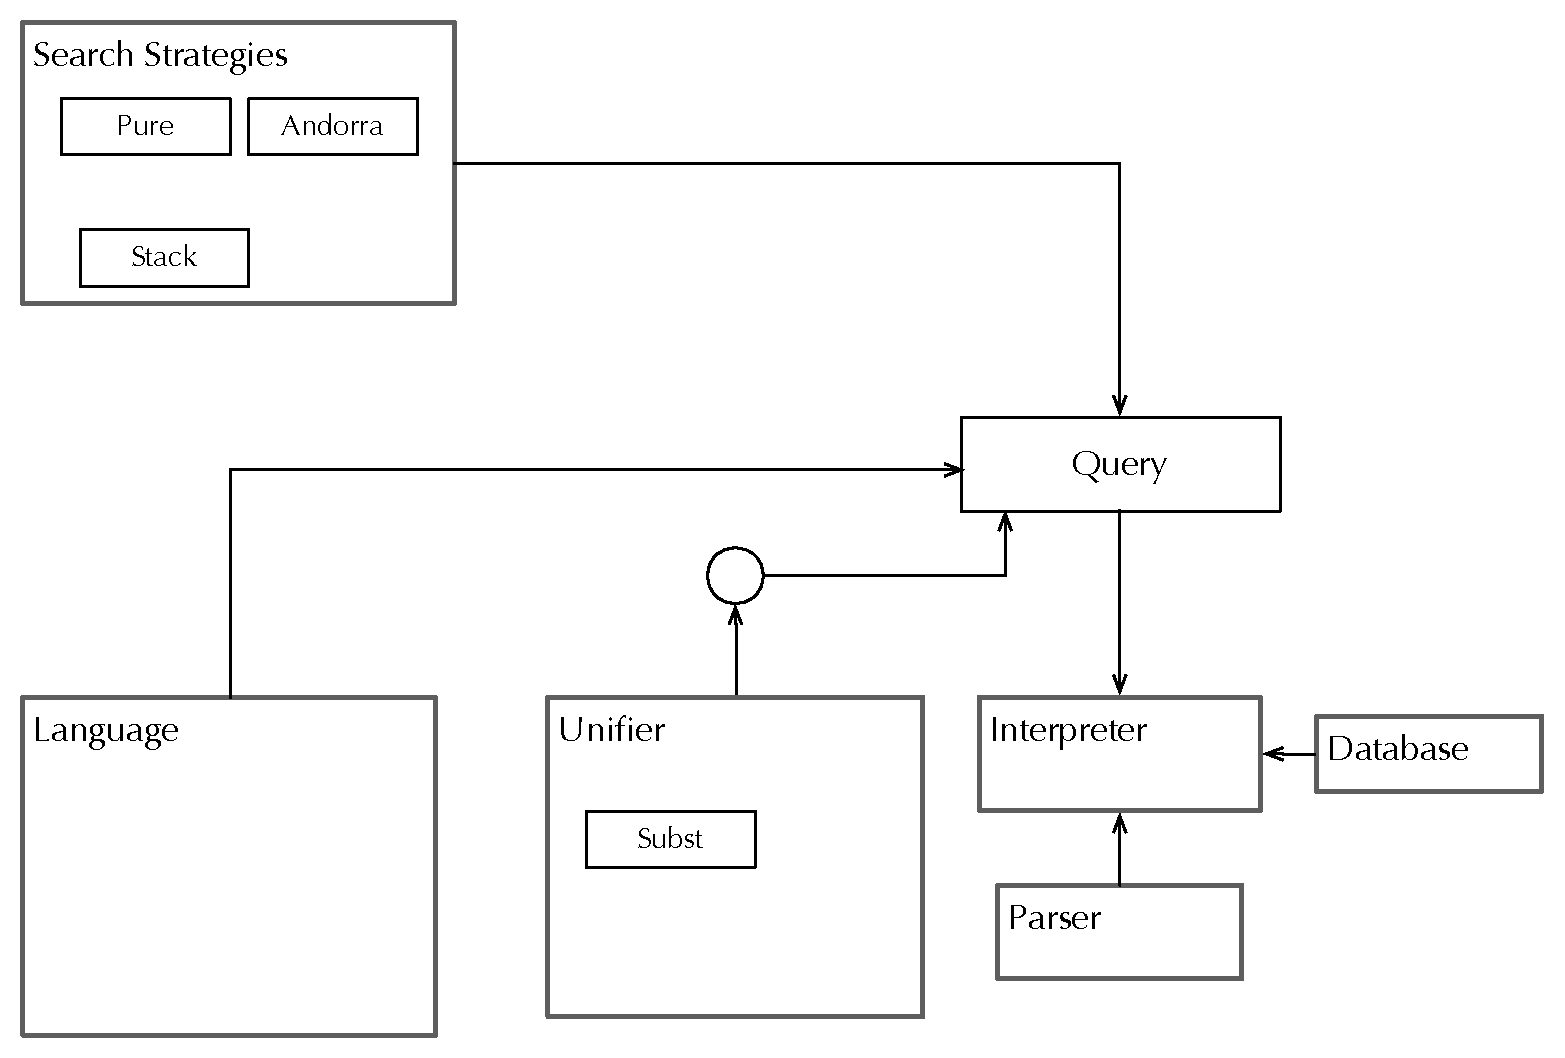
\includegraphics[width=1\textwidth]{Prototype-3-diagram.pdf}
\vspace*{-1cm}
  \caption{Architecture of Prototype 3}
  \label{fig:architecture-proto-3}
\end{figure}


\section{Section title needed}
When two terms are to be unified we can use Chapter~\ref{proto1},

\prologConstruct{term1} and \prologConstruct{term2} are matched and an assignment is the result 

now this may be a part of a query resolution procedure

to reach the point where two terms need to unified will happen through some sort of search strategy

and our approach is independent of that, and this prototype is a proof of concept to implementing query resolution using unification with
variable search strategy


\section{Unification}
The first, ``unification'' regards how terms are matched and variables assigned to make terms
match.
\cite{website:prologunification}



\section{Resolution}
this where the complete procedure takes place after the query is passed along with the knowledge 

the resolver searches to create and a list of  goals and then tries to achieve each one.

\cite{website:prologresolution}

\cite{website:resolutionlogicwiki}


\section{Backtracking}

\section{Search strategies}
The base implementation used for this prototype  is \cite{website:mini-prolog-hugs98} and below are the search
strategies
\subsection{Stack Engine}
\begin{singlespace}
\inputminted[linenos, firstline=29, lastline=62]{haskell}{haskell-proto3-sudsy-woe.hs}
\end{singlespace}

\subsection{Pure Engine}
\begin{singlespace}
\inputminted[linenos, firstline=26, lastline=46]{haskell}{haskell-proto3-absurd-silicon.hs}
\end{singlespace}

\subsection{Andorra Engine}
\begin{singlespace}
\inputminted[linenos, firstline=29, lastline=75]{haskell}{haskell-proto3-diatomic-unbank.hs}
\end{singlespace}

\section{Current Unification}
\begin{singlespace}
  \inputminted[linenos, firstline=65, lastline=82]{haskell}{haskell-proto3-pentyl-skater.hs}
\end{singlespace}


\section{Syntax Modification}
\begin{singlespace}
  \inputminted[linenos, lastline=352]{haskell}{haskell-proto3-uplift-apart.hs}
\end{singlespace}

\section{Monadic Unification}
\begin{singlespace}
  \inputminted[linenos]{haskell}{haskell-proto3-bevy-icebox.hs}
\end{singlespace}


\section{Chapter Recapitulation}
Recapitulating, this chapter provided us with a working implementation of a \progLang{Prolog}-like interpreter with the option to change
the search strategy further proving the modularity and genericity of the language modification and monadic unification procedure.

\end{document}
